\documentclass{beamer-control}
\usepackage{beamer-control-singlefile}
\INCLUDEONLY{Qualitative Analysis}
\begin{document}
\CONCEPT{Qualitative Analysis}

\begin{SUMMARY}
\begin{itemize}
\item Vector fields
\item Phase portraits
\item Equilibrium Points
\item Limit Cycles
\end{itemize}
\vfill References:
\begin{itemize}
\item \astrom{§5.2}
\end{itemize}
\printbibliography
\end{SUMMARY}



\SUBCONCEPT{Vector fields and Phase portraits}

\begin{frame}
\frametitle{ODE vector field}
Consider the ODE:
\begin{align}
\Deriv{x}{t} = F(x)
\end{align}
\begin{itemize}
\item At every $x$, $F(x)$ defines the `rate of change' of the system
\item We can \emph{plot} this rate of change as a function over state space
\item For a system with two state variables, this is planar plot with a 2D vector defined at all points on the plane
\item This plot is known as a \emph{vector field plot}, or \emph{quiver} plot (\texttt{quiver()} in Matlab)
\end{itemize}
\end{frame}

\begin{frame}
\frametitle{ODE vector field plot}
\framesubtitle{Note the positions of zero vector}
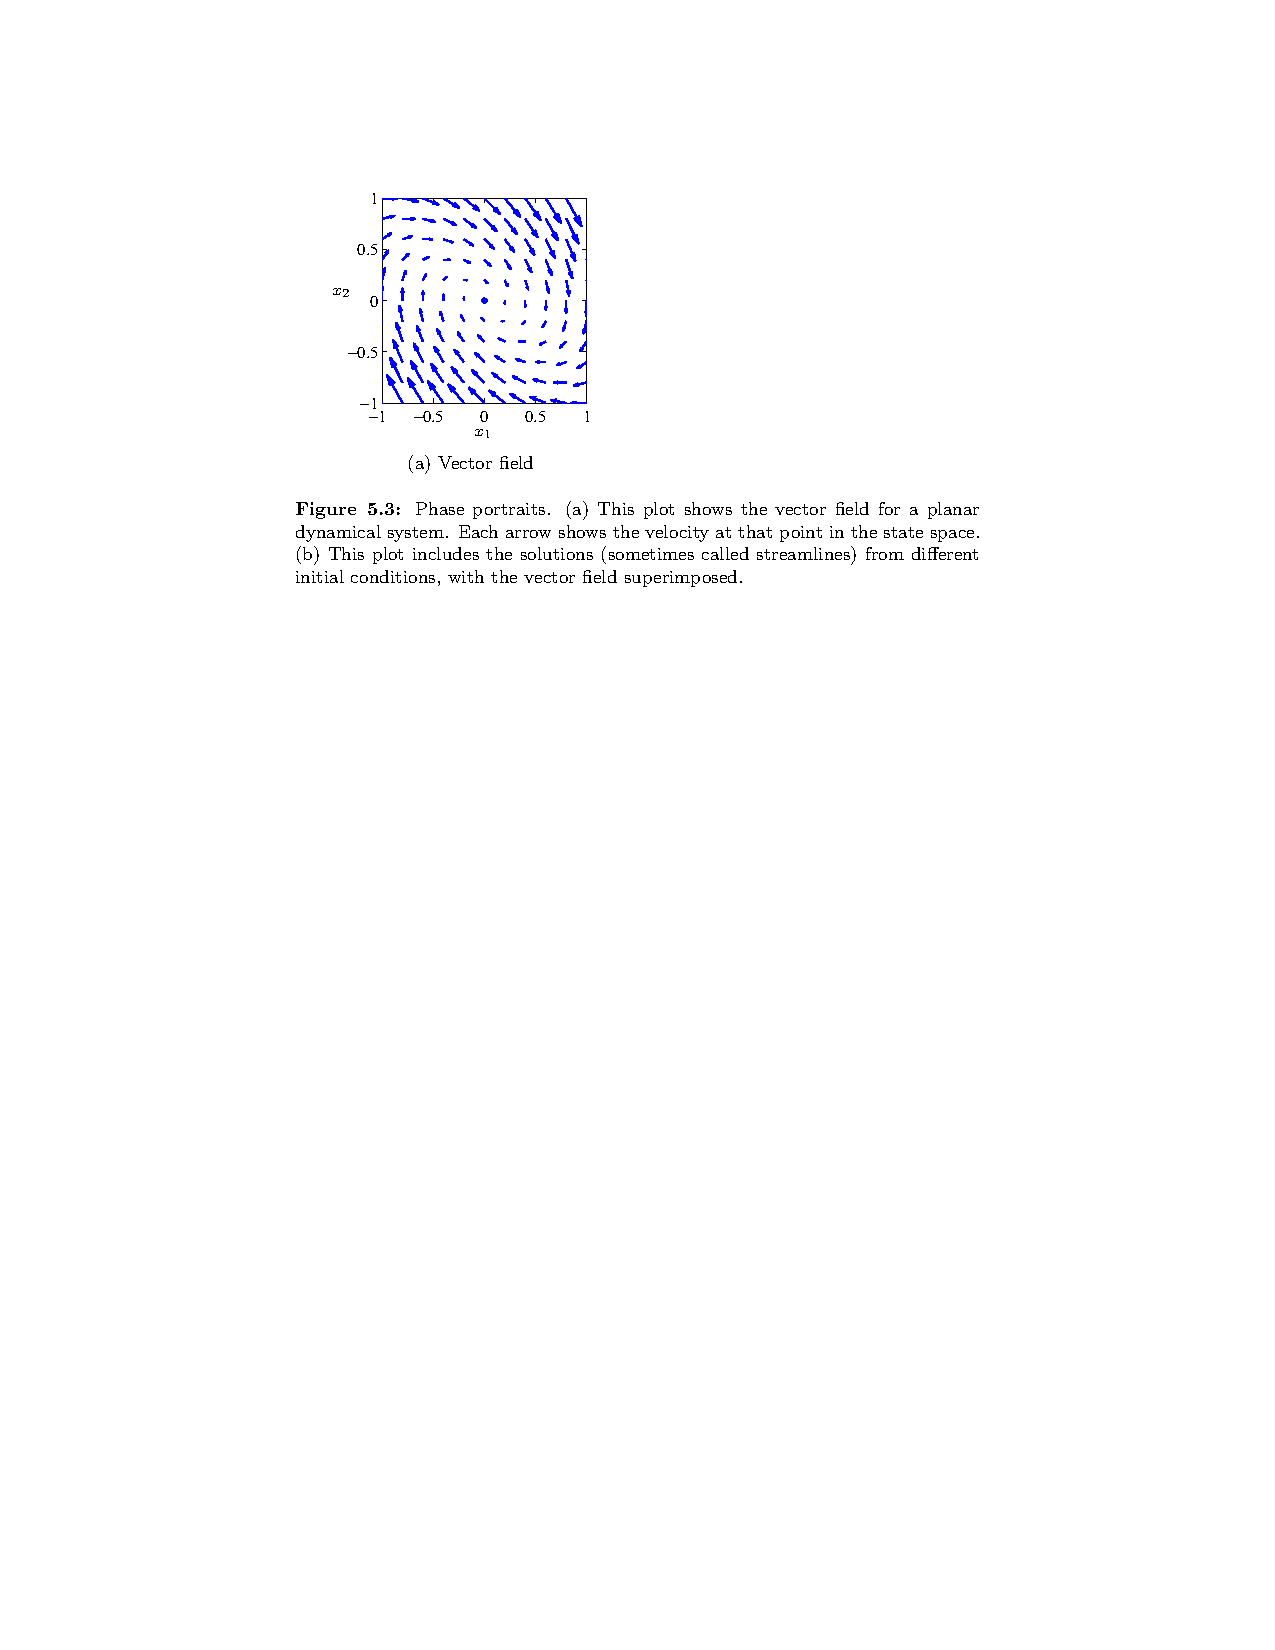
\includegraphics[width=\linewidth]{figure5.3a}
\end{frame}

\begin{frame}
\frametitle{Phase portrait}
\begin{itemize}
\item The vector field is best at highlighting stationary points
\item You can infer but can't directly visualise trajectories
\item Enter the `phase portrait' --- a superimposed collection of trajectories 
\item Where the trajectories cluster and converge tells us important properties of the system
\item Note that trajectories don't tell us rate of change
\end{itemize}
\end{frame}

\begin{frame}
\frametitle{Phase portrait plot}
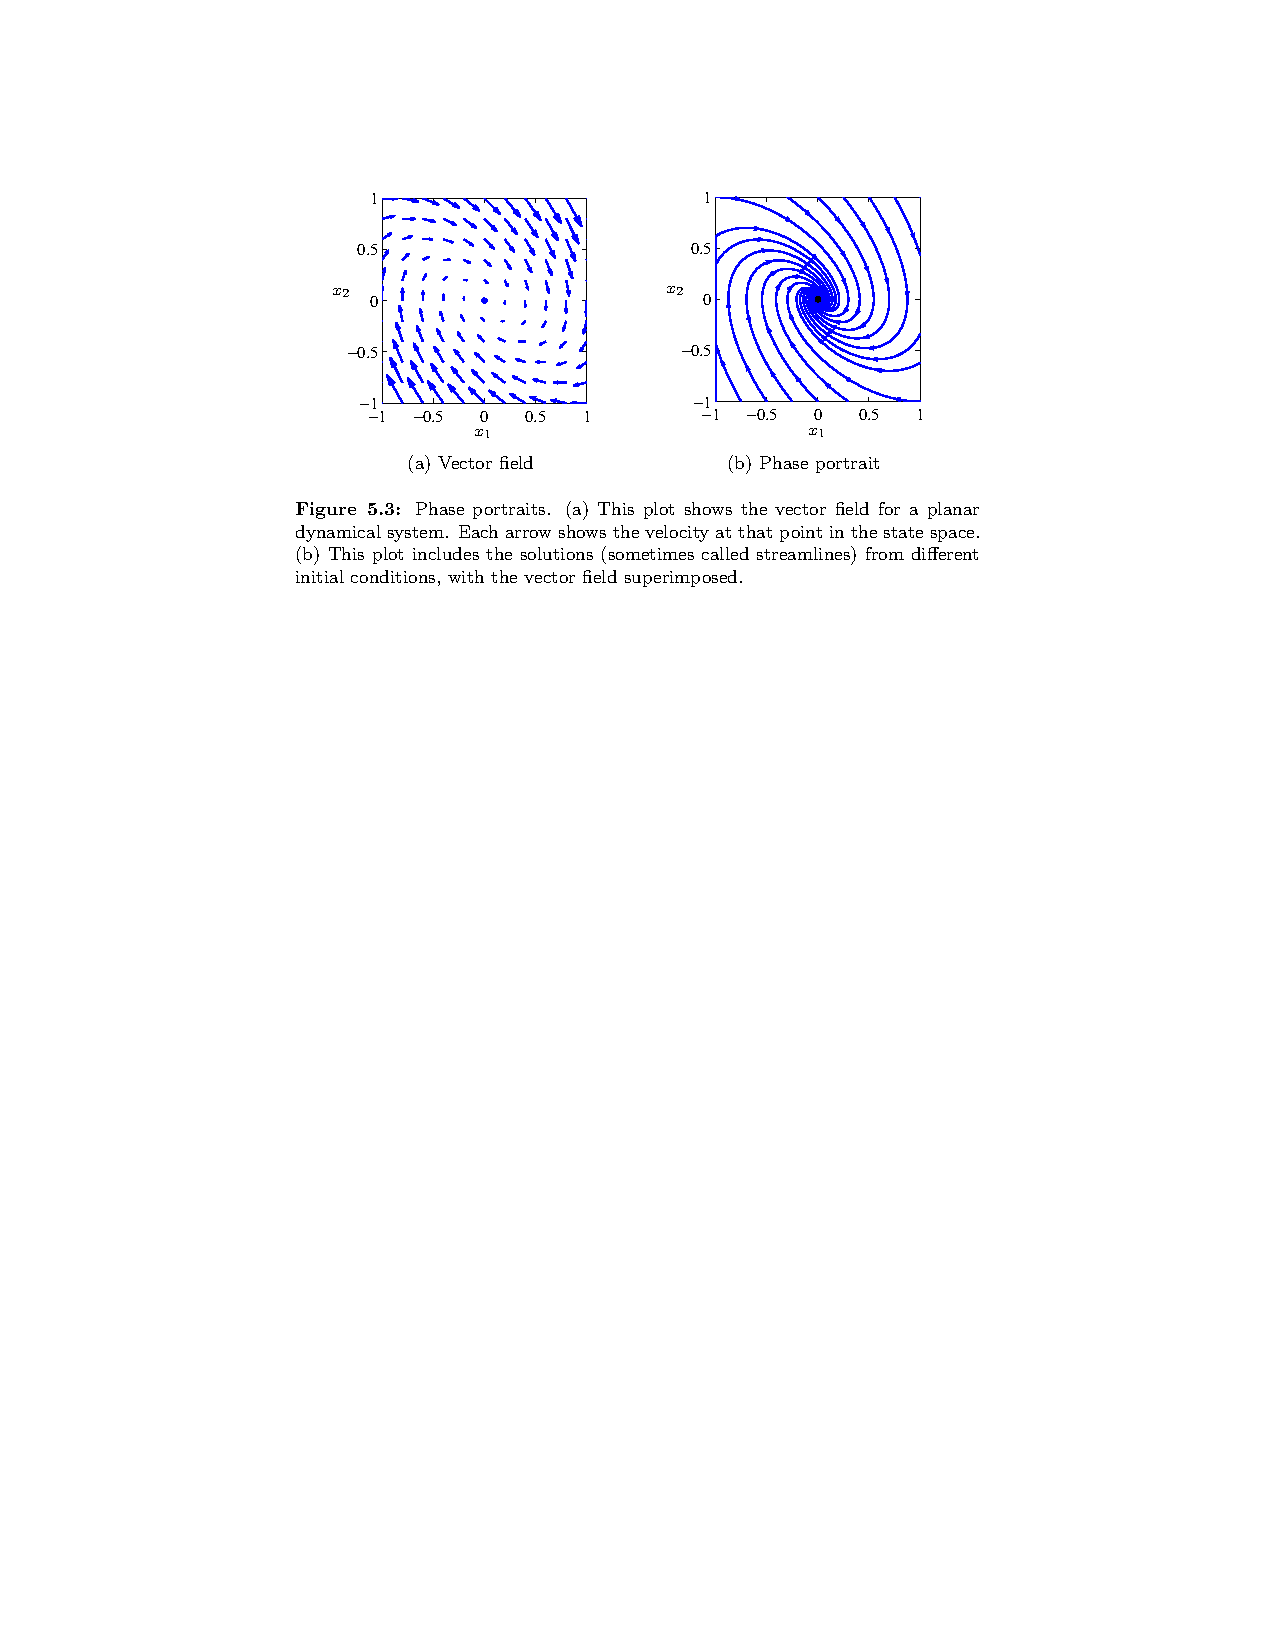
\includegraphics[width=\linewidth]{figure5.3b}

\end{frame}

\SUBCONCEPT{Equilibrium Points and Limit Cycles}

\begin{frame}{Equilibrium point}
For dynamical system $\Deriv{x}{t} = F(x)$, an equilibrium point $x_e$ is:
\begin{align}
\left.\Deriv{x}{t}\right|_{x=x_e} &= F(x_e) = 0
\end{align}
Qualitatively:
\vspace{3cm}
\end{frame}

\begin{frame}
\frametitle{Inverted pendulum equilibria}
This is a second order system with state vector
\begin{gather}
x = \Matr{x_1\\x_2} = \Matr{\theta\\\dot\theta}
\end{gather}
After normalising away constants:
\begin{gather}
\Deriv{x}{t} = \Matr{\dot x_1\\\dot x_2} = \Matr{\dot\theta\\\ddot\theta} = \Matr{\dot\theta\\\sin\theta-c\dot\theta+{\color{red}u\cos\theta}}
\end{gather}
When is $\Deriv{x}{t} = \Matr{0\\0}$ ?

\end{frame}

\begin{frame}
\frametitle{Inverted pendulum equilibria}
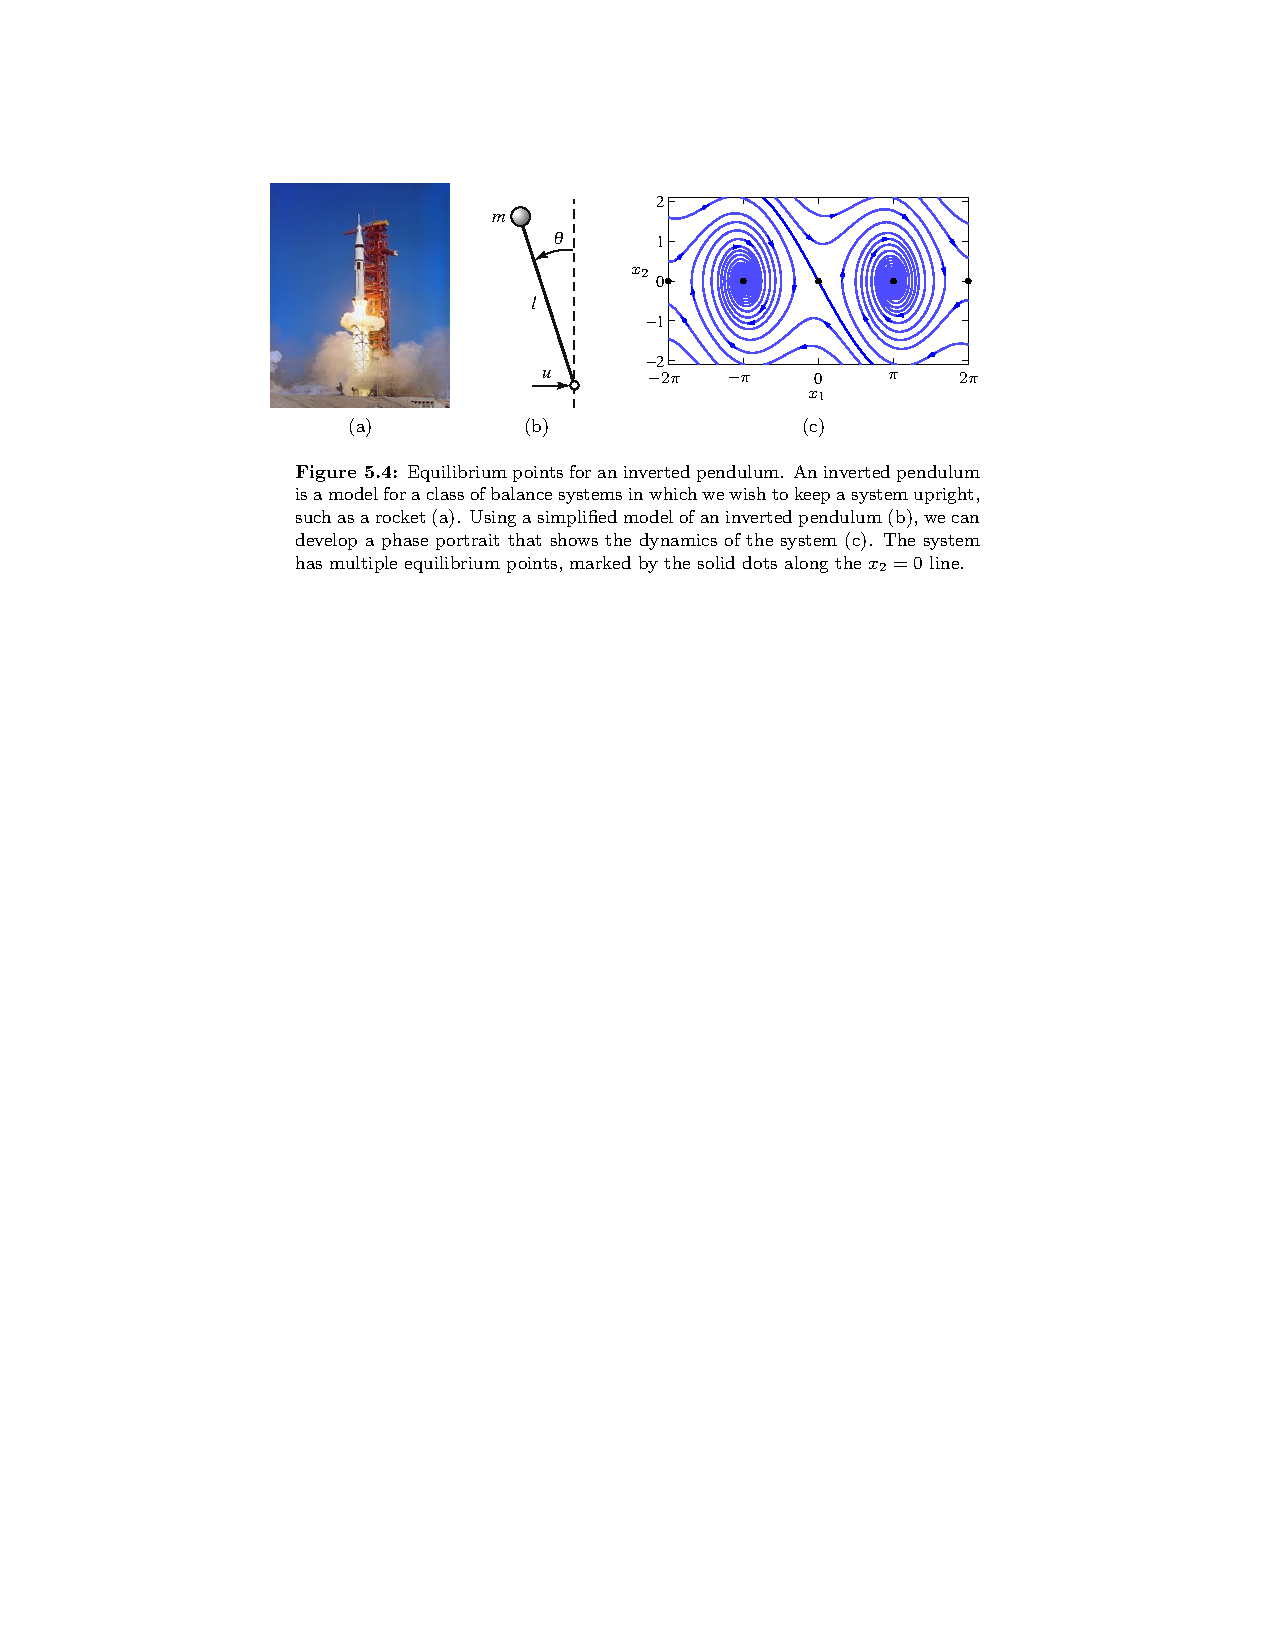
\includegraphics[width=\linewidth]{figure5.4}

\end{frame}

\begin{frame}
\frametitle{Limit cycles}
\framesubtitle{Example of an electronic oscillator}
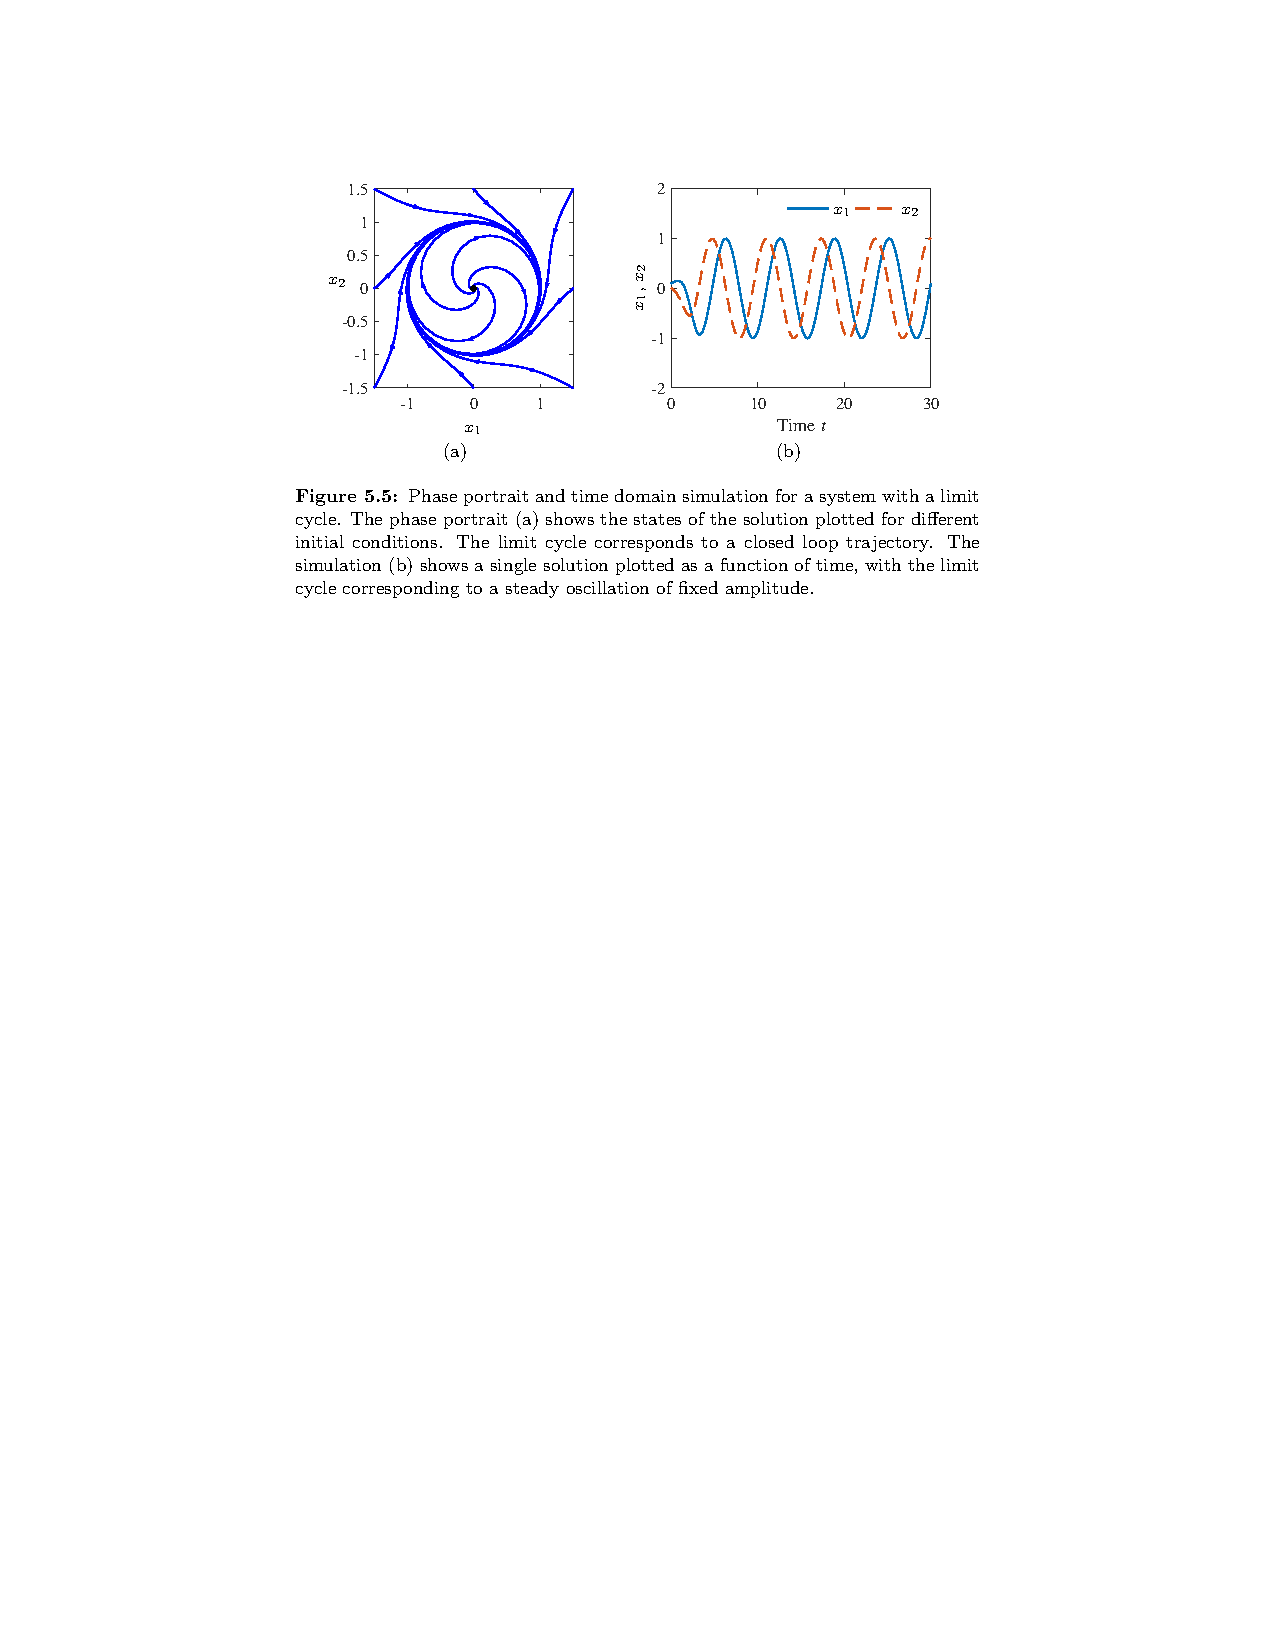
\includegraphics[width=\linewidth]{figure5.5}

\end{frame}

\begin{frame}
\frametitle{Physical system with limit cycle}
\framesubtitle{\minicite{cheffer2021-amm}}

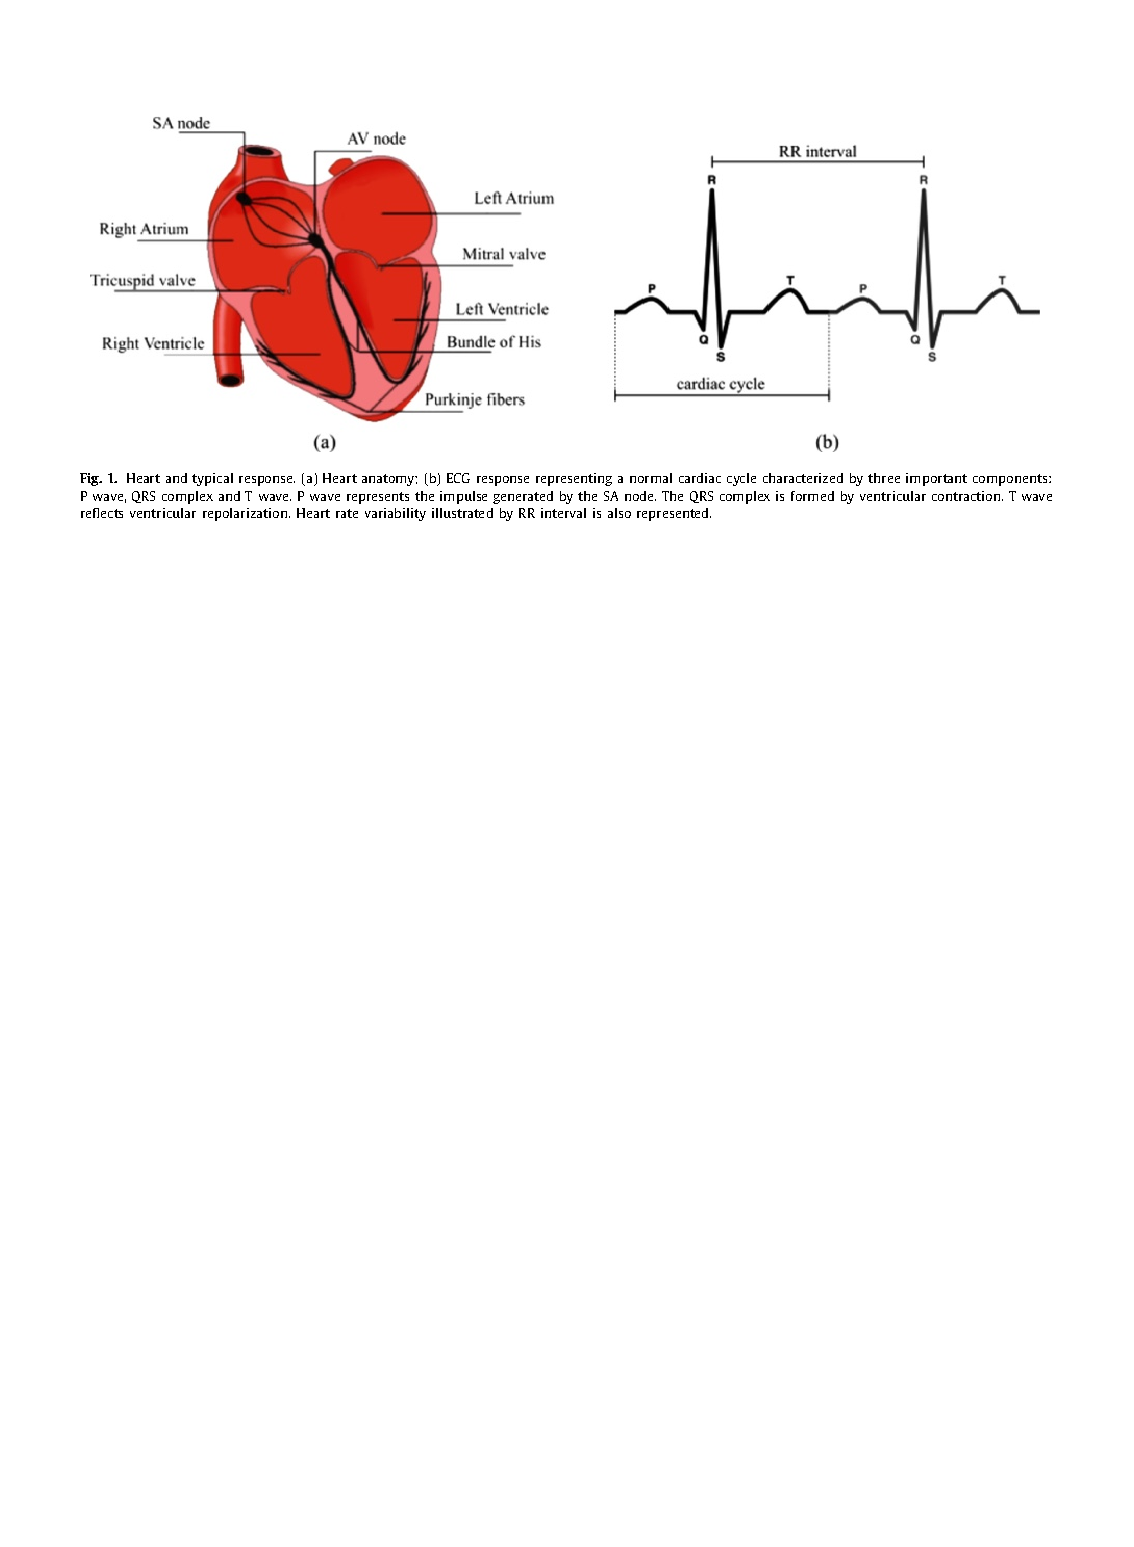
\includegraphics[width=\linewidth]{cheffer2021-fig1}

\end{frame}

\begin{frame}
\frametitle{Physical system with limit cycle}
\framesubtitle{\minicite{cheffer2021-amm}}

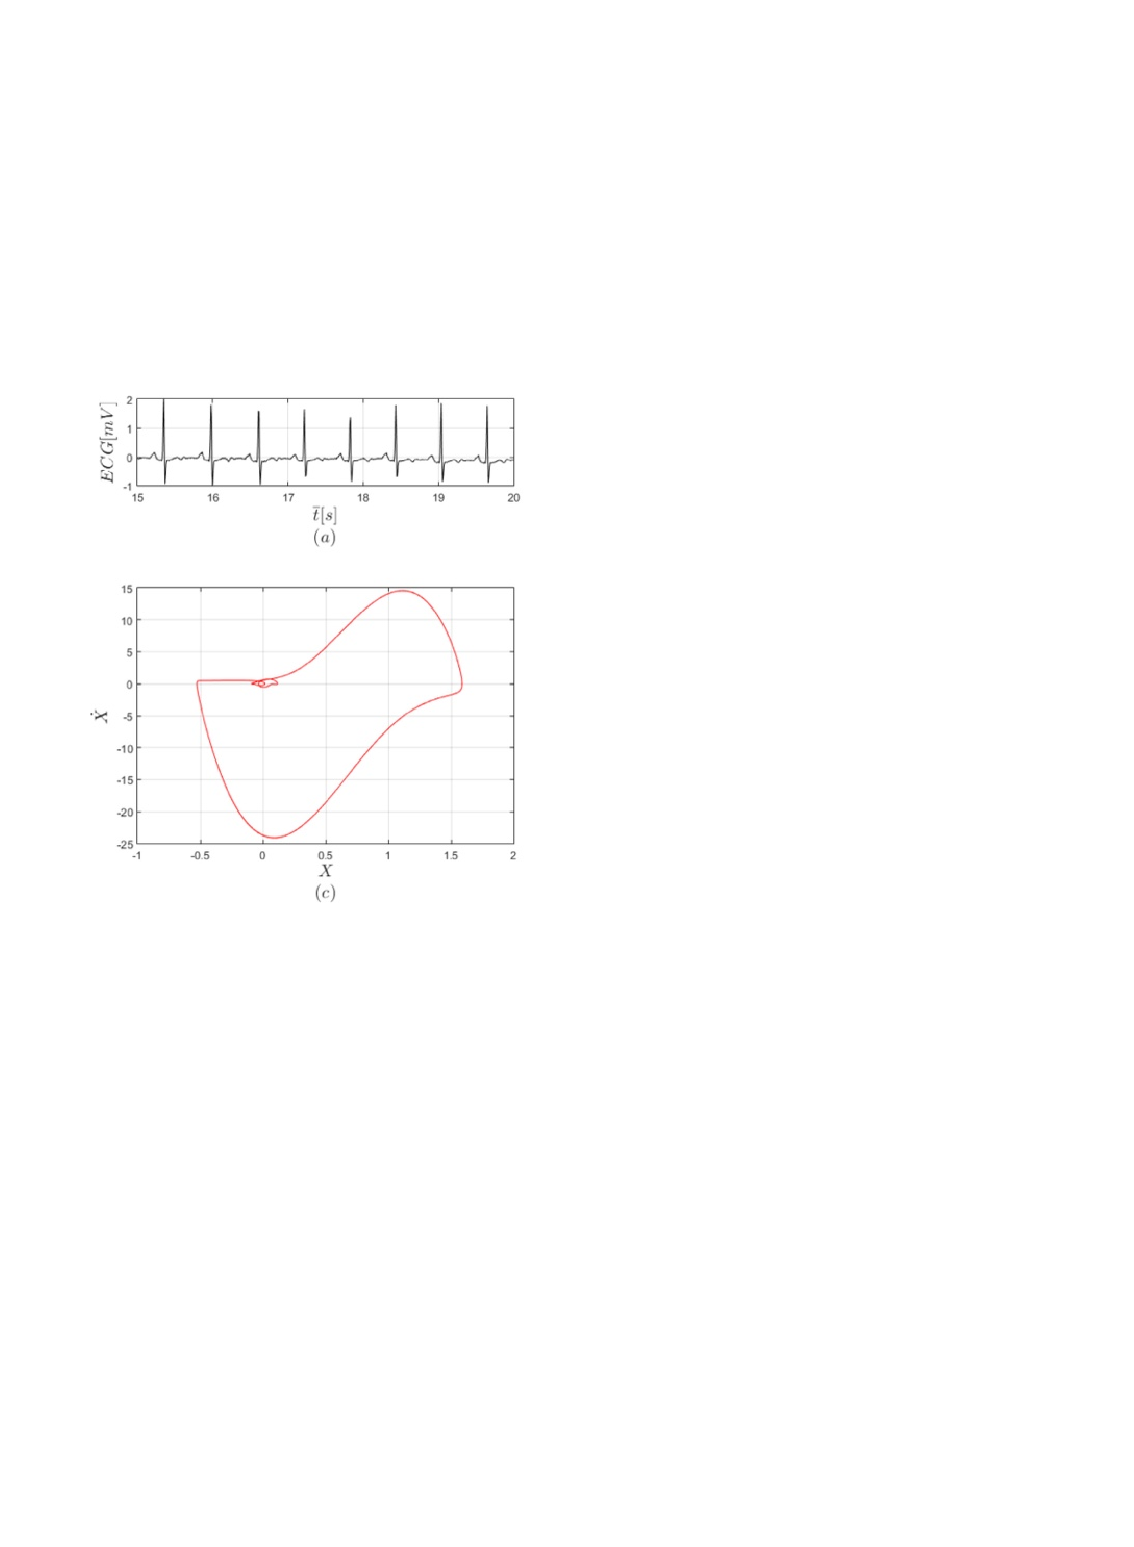
\includegraphics[width=0.45\linewidth]{cheffer2021-fig4}\hfil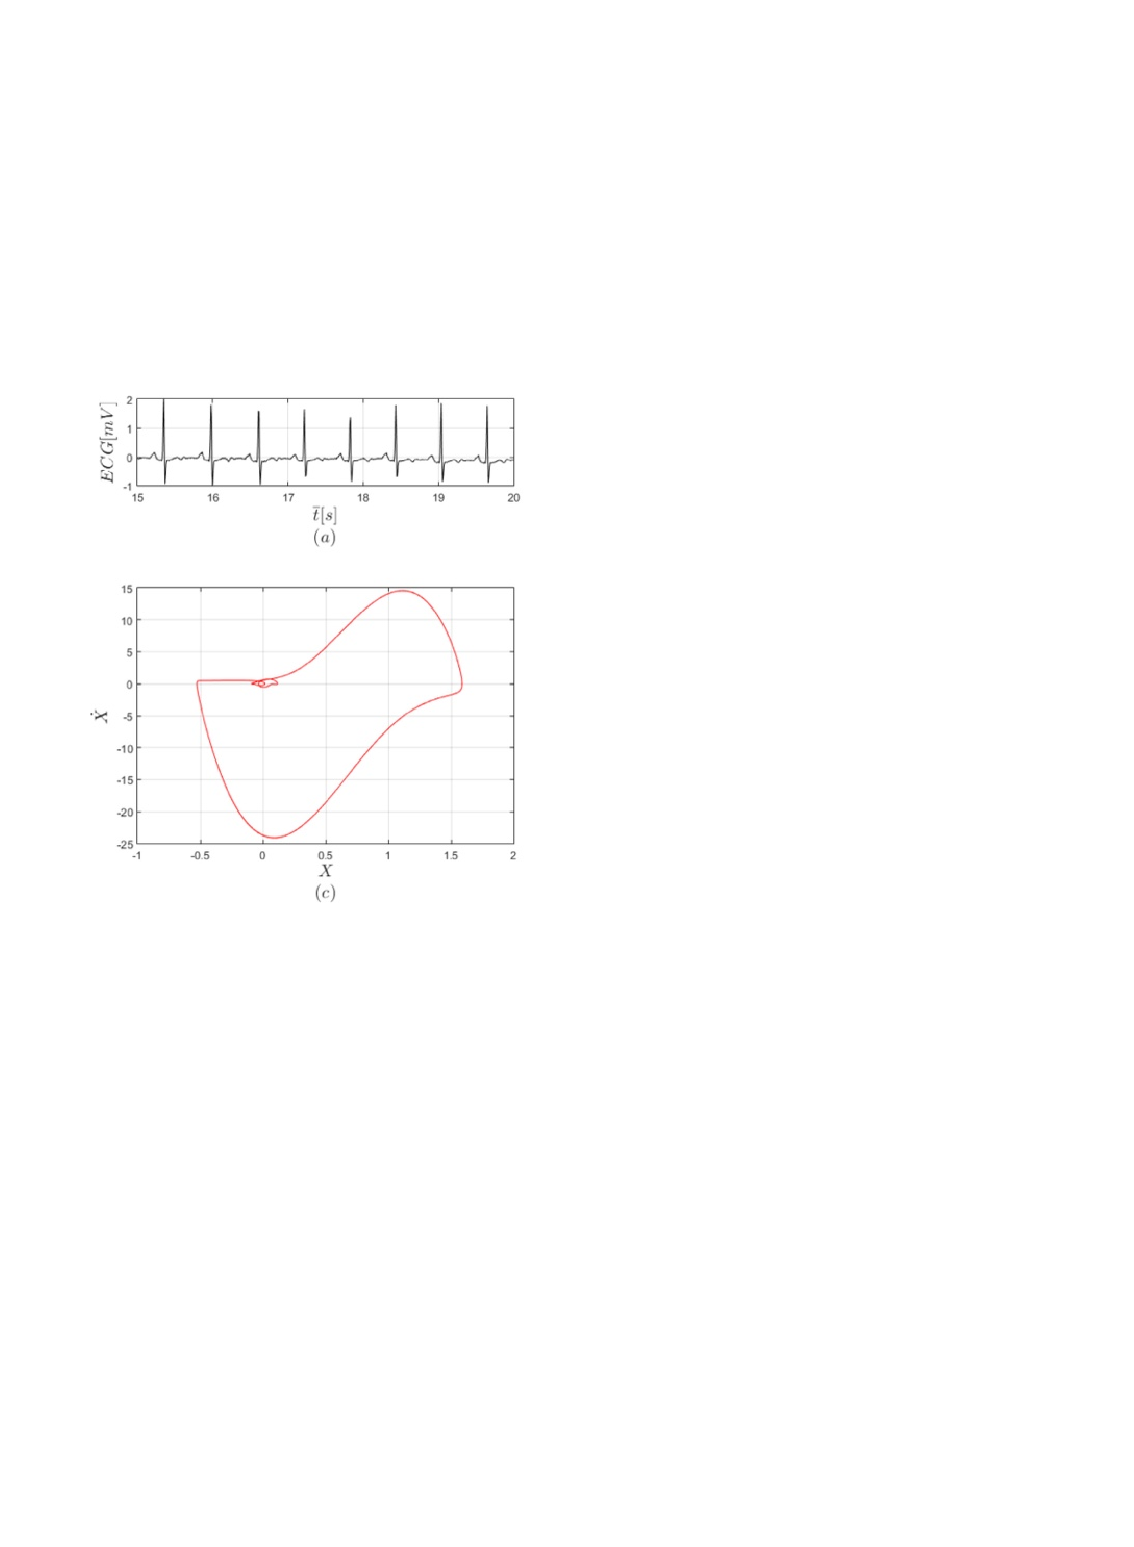
\includegraphics[width=0.45\linewidth]{cheffer2021-fig4}


\end{frame}

\begin{frame}
\frametitle{More complex dynamics example}
\framesubtitle{\minicite{bizyaev2024-rcd}}

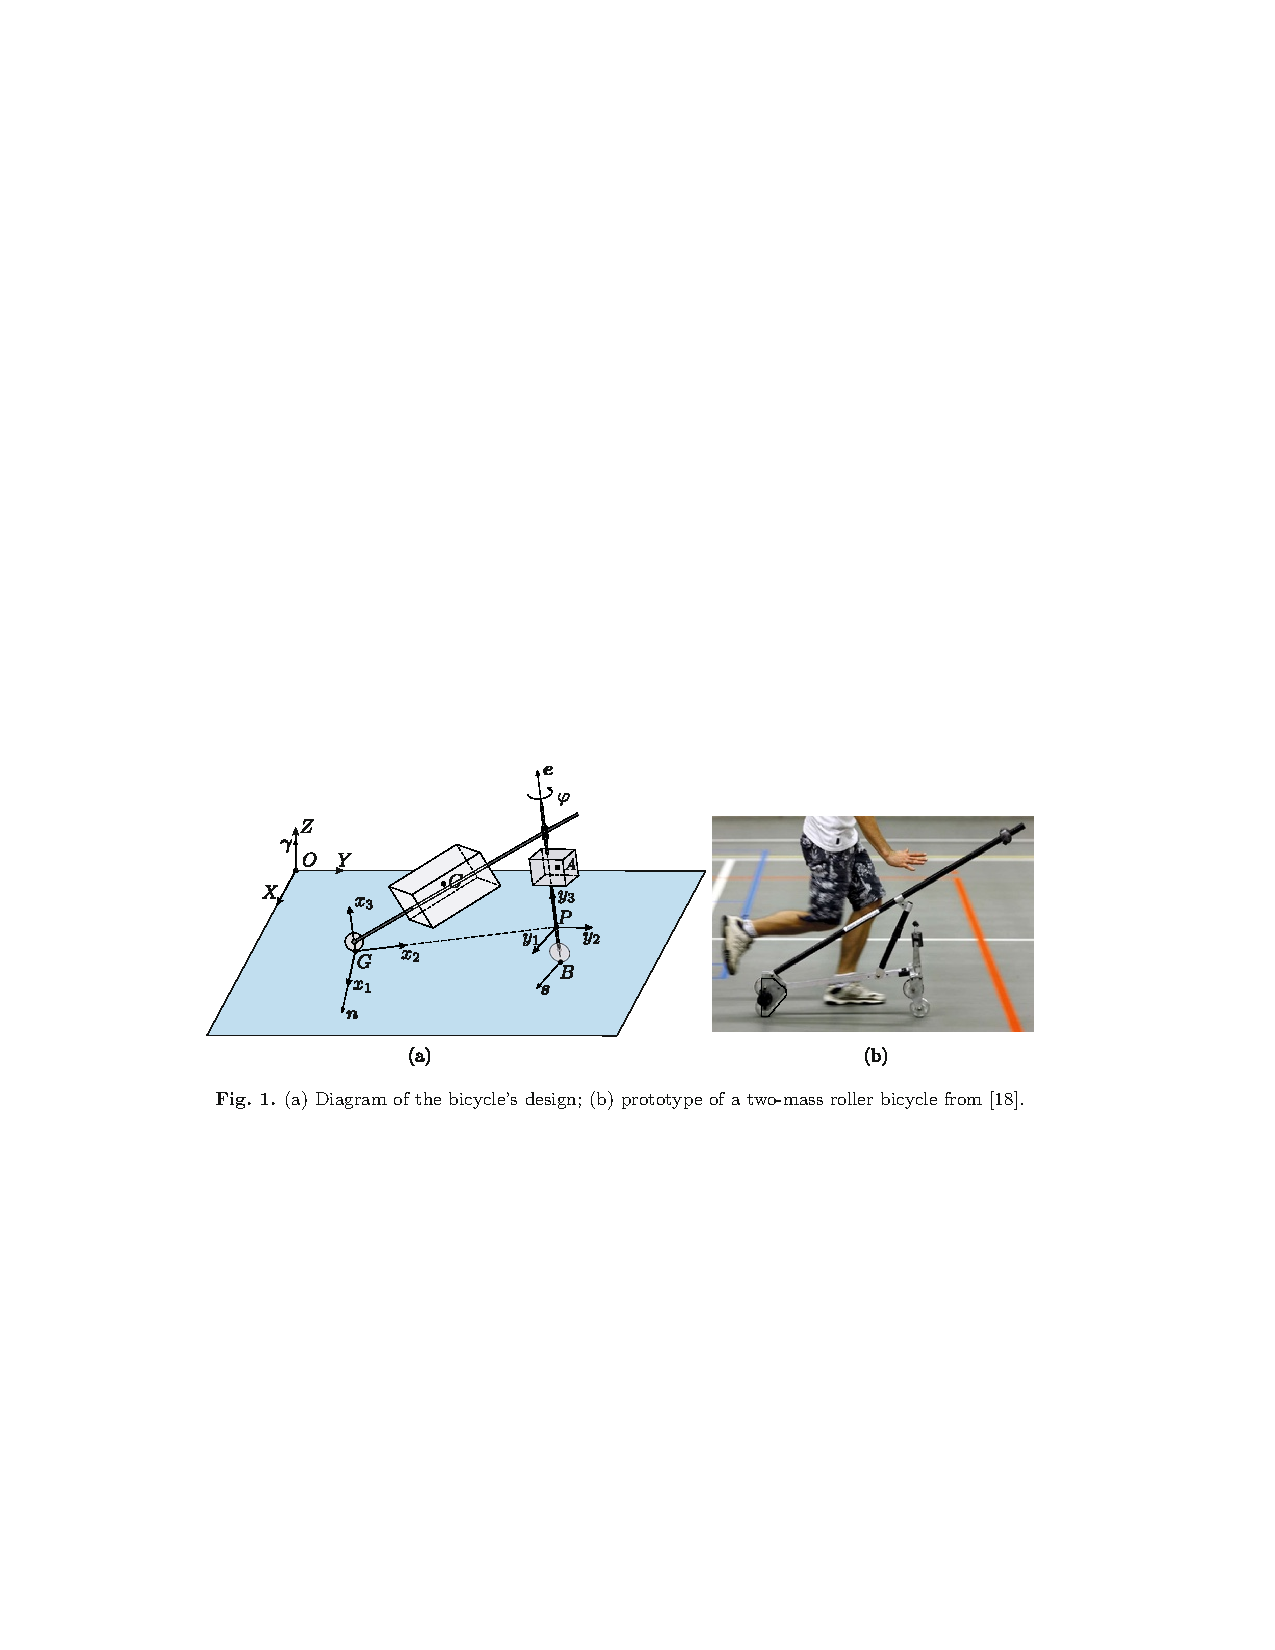
\includegraphics[width=\linewidth]{bizyaev2024-fig1}

\end{frame}

\begin{frame}
\frametitle{More complex dynamics example}
\framesubtitle{\minicite{bizyaev2024-rcd}}

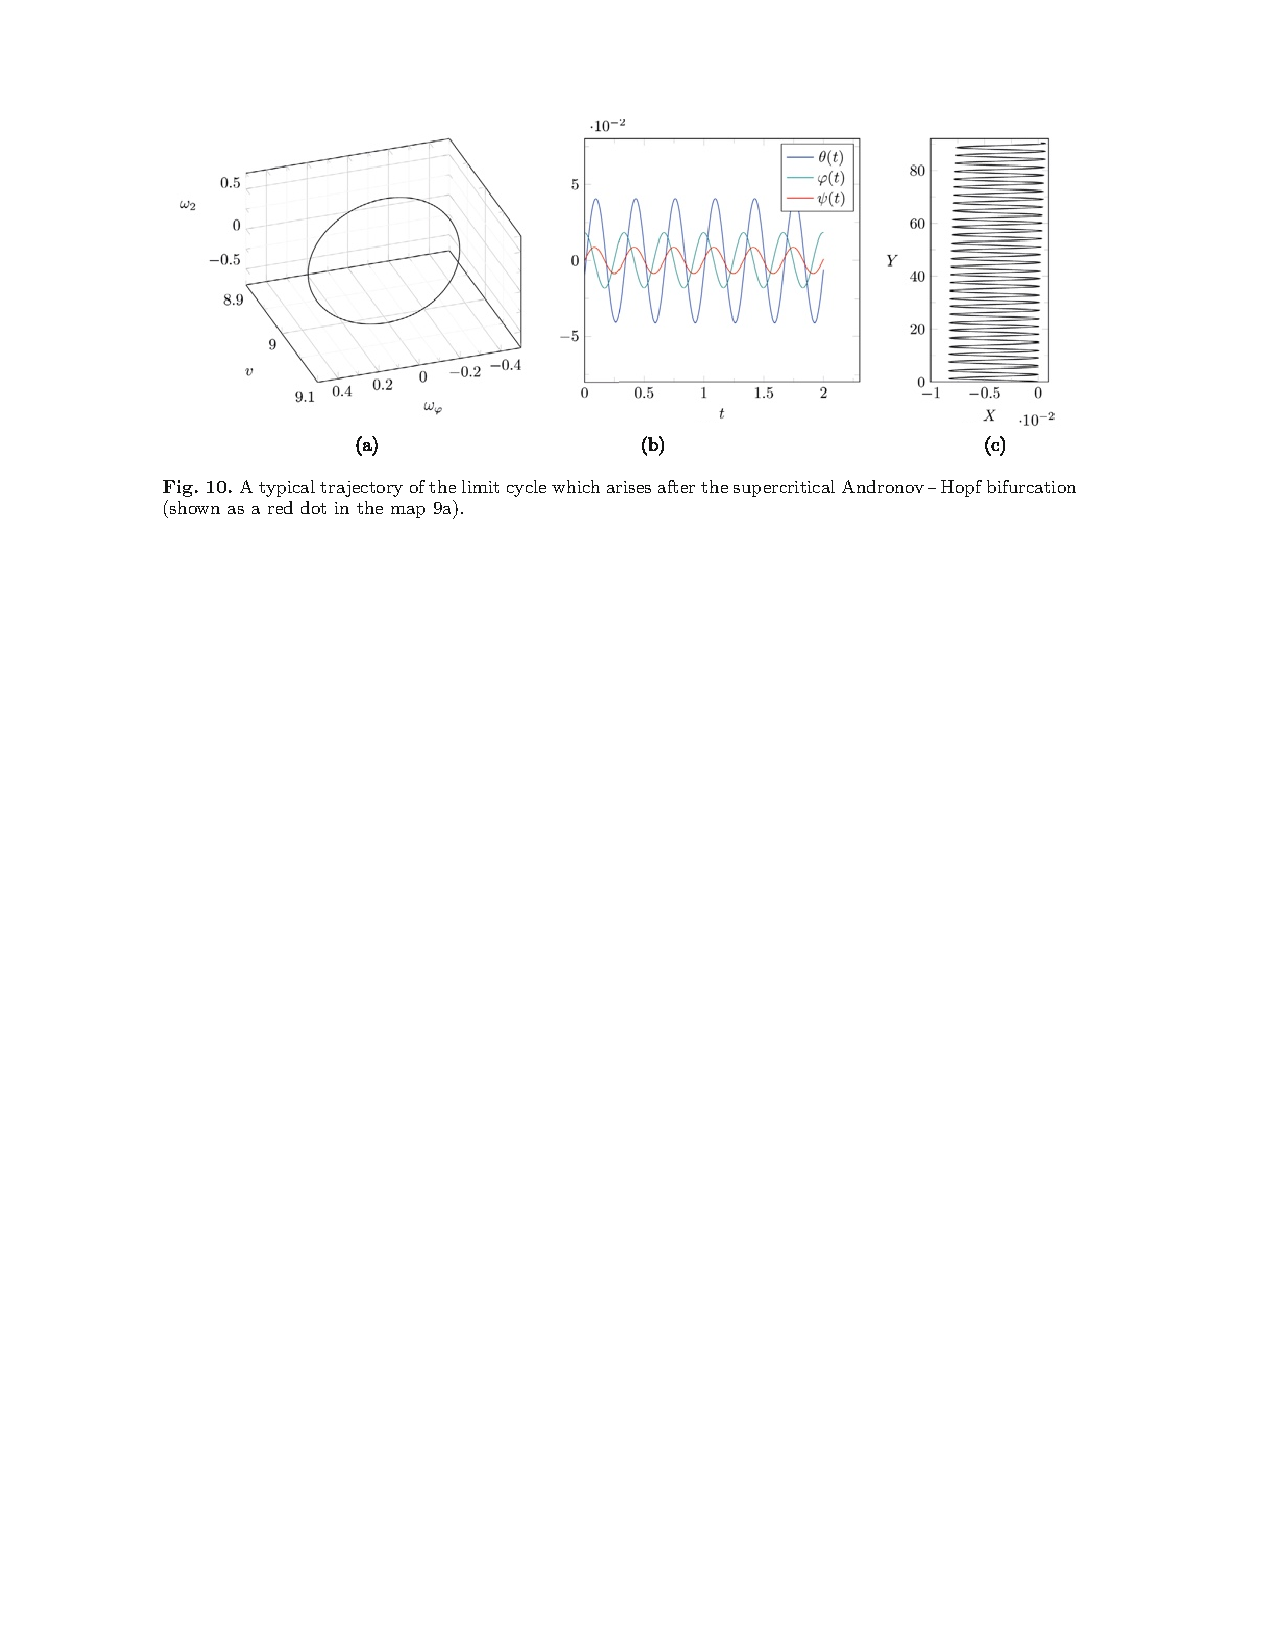
\includegraphics[width=\linewidth]{bizyaev2024-fig10}

\end{frame}


\SUMMARYFRAME
\FINALE

\end{document}
